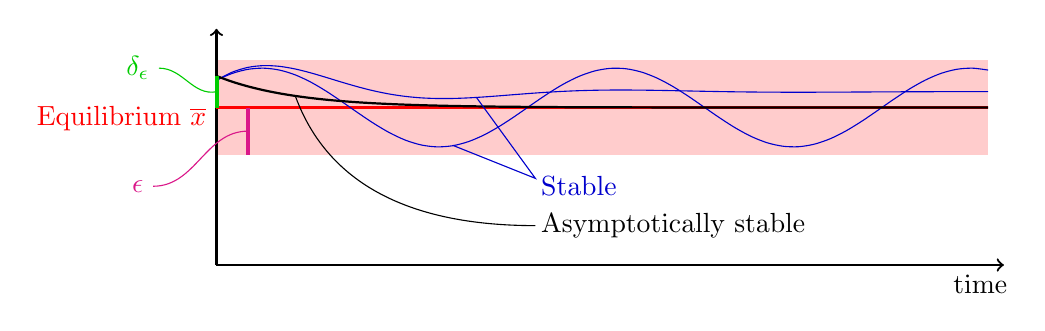
\begin{tikzpicture}

\draw[draw=none,fill=red!20!white]
     (0,1.4) rectangle (9.8,2.6);

\draw[->,thick](0,0)
     -- node[pos=0.97,below]{time}
     (10,0);
\draw[->,thick](0,0) -- (0,3);

\draw[red, thick] (0,2)
     -- node[pos=0,left,yshift=-4]
     {Equilibrium $\overline{x}$}
     (9.8,2);

\draw[smooth,blue!80!black,
      samples=50,domain=0:9.8,variable=\t]
      plot({\t},
           {2.2+0.53*sin(80*(\t+0.2))
                    *exp(-0.6*\t)});
\draw[smooth,blue!80!black,
      samples=50,domain=0:9.8,variable=\t]
      plot({\t},
           {2+0.5*sin(80*(\t+0.55))});
\draw[smooth,black,thick,
      samples=50,domain=0:9.8,variable=\t]
      plot({\t},
           {2+0.4*exp(-\t)});

\node[blue!80!black,anchor=west]
     at (4,1) (sCap)
     {Stable};
\draw[blue!80!black]
     (3,1.52) -- (4.05,1.1) -- (3.3,2.13);

\node[black,anchor=west]
     at (4,0.5) (asCap)
     {Asymptotically stable};
\draw[black]
     (1,2.15)
     to [out=-70,in=180] (4.05,0.5);

\draw[magenta!90!black,ultra thick]
     (0.4,2) --++ (0,-0.6);
\node[magenta!90!black]
     at (-1,1) (eCap) {$\epsilon$};
\draw[magenta!90!black]
     (0.4,1.7)
     to [out=180,in=0] (eCap.east);

\draw[green!80!black,ultra thick]
     (0.01,2) --++ (0,0.4);
\node[green!80!black]
     at (-1,2.5) (deCap)
     {$\delta_{\epsilon}$};
\draw[green!80!black]
     (0,2.2)
     to [out=190,in=0] (deCap.east);

\end{tikzpicture}